\documentclass[border=4pt]{standalone}
\usepackage{fontspec}
\usepackage{amsmath}
\usepackage{unicode-math}
\setmainfont{Latin Modern Roman}
\setmathfont{Latin Modern Math}
\usepackage{pgfplots}
\usepackage{pgfplotstable}
\pgfplotsset{compat=1.18}
\usepackage{tkz-euclide}
\usetikzlibrary{arrows.meta,calc,angles,quotes,patterns,3d,backgrounds}
\definecolor{ink}{HTML}{123428}
\definecolor{asy}{HTML}{475569}
\definecolor{mint}{HTML}{86e0bd}
\tikzset{asym/.style={asy, line width=0.9pt, dash pattern=on 5pt off 3.5pt},
         guide/.style={gray!70, line width=0.6pt, densely dotted},
         dot/.style={circle, inner sep=0pt, minimum size=5pt, draw=white, line width=0.5pt},
         odot/.style={circle, inner sep=0pt, minimum size=5.5pt, fill=white, line width=1pt},
         lab/.style={font=\footnotesize, inner sep=1.5pt, text=ink}}
\begin{document}
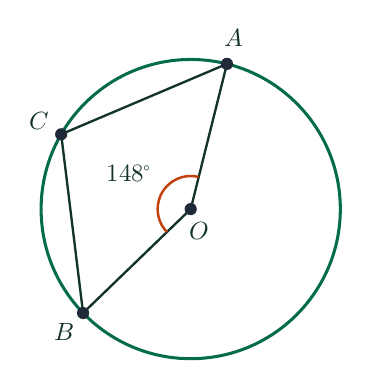
\begin{tikzpicture}
\draw[color={rgb,255:red,4;green,107;blue,77}, line width=1.1pt] (0,0) circle (1.900);
\draw[ink, line width=0.85pt] (-1.645,0.950) -- (0.460,1.844);
\draw[ink, line width=0.85pt] (-1.645,0.950) -- (-1.367,-1.320);
\draw[ink, line width=0.85pt] (0.000,0.000) -- (0.460,1.844);
\draw[ink, line width=0.85pt] (0.000,0.000) -- (-1.367,-1.320);
\draw[color={rgb,255:red,194;green,65;blue,12}, line width=0.9pt] (0.102,0.408) -- (0.048,0.417) -- (-0.006,0.420) -- (-0.060,0.416) -- (-0.113,0.405) -- (-0.164,0.387) -- (-0.213,0.362) -- (-0.257,0.332) -- (-0.298,0.296) -- (-0.334,0.255) -- (-0.364,0.210) -- (-0.388,0.161) -- (-0.405,0.110) -- (-0.416,0.057) -- (-0.420,0.003) -- (-0.417,-0.051) -- (-0.407,-0.104) -- (-0.390,-0.156) -- (-0.367,-0.205) -- (-0.337,-0.250) -- (-0.302,-0.292);
\node[font=\small, text=ink, inner sep=0.5pt, fill=white] at (-0.779,0.450) {$148^\circ$};
\fill[color={rgb,255:red,31;green,41;blue,55}] (0.460,1.844) circle (2.2pt);
\fill[color={rgb,255:red,31;green,41;blue,55}] (-1.367,-1.320) circle (2.2pt);
\fill[color={rgb,255:red,31;green,41;blue,55}] (-1.645,0.950) circle (2.2pt);
\fill[color={rgb,255:red,31;green,41;blue,55}] (0.000,0.000) circle (2.2pt);
\node[font=\small, text=ink, inner sep=0.5pt] at (0.542,2.173) {$A$};
\node[font=\small, text=ink, inner sep=0.5pt] at (-1.611,-1.556) {$B$};
\node[font=\small, text=ink, inner sep=0.5pt] at (-1.940,1.120) {$C$};
\node[font=\small, text=ink, inner sep=0.5pt] at (0.103,-0.282) {$O$};
\end{tikzpicture}
\end{document}
